\documentclass{ctexart}
\usepackage{amsmath}
\usepackage{float}
\usepackage{amssymb}
\usepackage{graphicx}
\usepackage{gbt7714}
\usepackage{pifont}
\usepackage{wrapfig}
\ctexset{
    % 修改 section。
    section={   
        name={,、},
        number={\chinese{section}}
    }
}

\title{示波器的调整和使用}
\author{陆知辰-10225301478}
\date{\today}
\graphicspath{{figure/}}

\begin{document}

\begin{titlepage}
  \centering
  % 插入图片
  
\includegraphics[width=0.5\textwidth]{ecnu.png}
  
  % 空行用于调整标题位置
  \vspace*{\baselineskip}
  
  % 标题
  \Huge\textbf{物\quad 理\quad 实\quad 验 \quad (二)}
  % 空行用于调整标题和其他信息之间的间距
  \vspace*{0.3\baselineskip}
  
  % 具体实验名称
  \huge 示波器的调整和使用
  
  % 空行用于调整时间和其他信息之间的间距
  \vspace*{2\baselineskip}
  
  % 时间
  \large 时间:\today
  
  % 空行用于调整时间和其他信息之间的间距
  \vspace*{\baselineskip}
  
  % 创作人
  \large 创作人:陆知辰
  
  % 空行用于调整创作人和学号之间的间距
  \vspace*{\baselineskip}
  
  % 学号
  \large 学号:10225301478
  
\end{titlepage}
\newpage
\tableofcontents
\newpage
\section{实验摘要}
  \subsection{实验概要}
  示波器是一种能观察各种电信号波形并可测量其电压、预率等的电子测量仪器,
  示波器还能对一些能转换成电信号的非电学量进行观测,因而它还是一种应用非常广泛的、通用的电子显示器。

  1897年德国物理学家发明了世界上第一台阴极射线管示波器.他出于好奇向阴极射线管的水平偏转片施加一个振荡信号,
  然后向纵向偏转片发送一个测试信号,结果在小荧光屏上产生瞬态的电波图像。这一发明逐步发展成一台测量仪器,
  并且其性能在后续的50多年里不断改善。1947年泰克公司的工程师霍华德·卫林实现了示波器的实用化和商业化。直到现在,
  示波器演变出了模拟示波器、数字示波器、混合示波器等种类,并广泛应用于信号测量、通信等各行各业。示波器原理上只应用了简单的物理理论,
  但却创造了了不起的成就并广泛应用至今。
  \subsection{实验目的}
  1.\quad 了解示波器的结构和示波器的示波原理。

  2.\quad 掌握示波器的使用方法,学会用示波器观察各种信号的波形。
  
  3.\quad 学会用示波器测量正弦交流信号电压。

  4.\quad 观察李萨如图,学会测量正弦信号频率的方法。

\section{实验原理}
示彼器有模拟示器与数字示器两种类型。两种示波器在结构上有相同之处,也存在着很大的差别。
从本质上来说,模拟示波器相当于用输入的信号直接驱动显示器,以便在示波器上显示信号波形,
并进行测量;数字示波器则是通过模数换把待测量的模拟信号转换为数字信号,它捕获的是一系列的样值,并对样值进行存储,随后再重构波形。

以下首先基于模拟示波器介绍示波器的工作原理,最后再介绍数字示波器。
  \subsection{模拟示波器的基本结构}
  图\ref{monijiegou}是模拟示波器的结构示意图,它主要是由示波管、X轴与Y轴衰减器和放大器、锯齿波发生器、
  同步触发电路和电源等几部分组成。

  \begin{figure}[bt]\label{monijiegou}
    \centering
    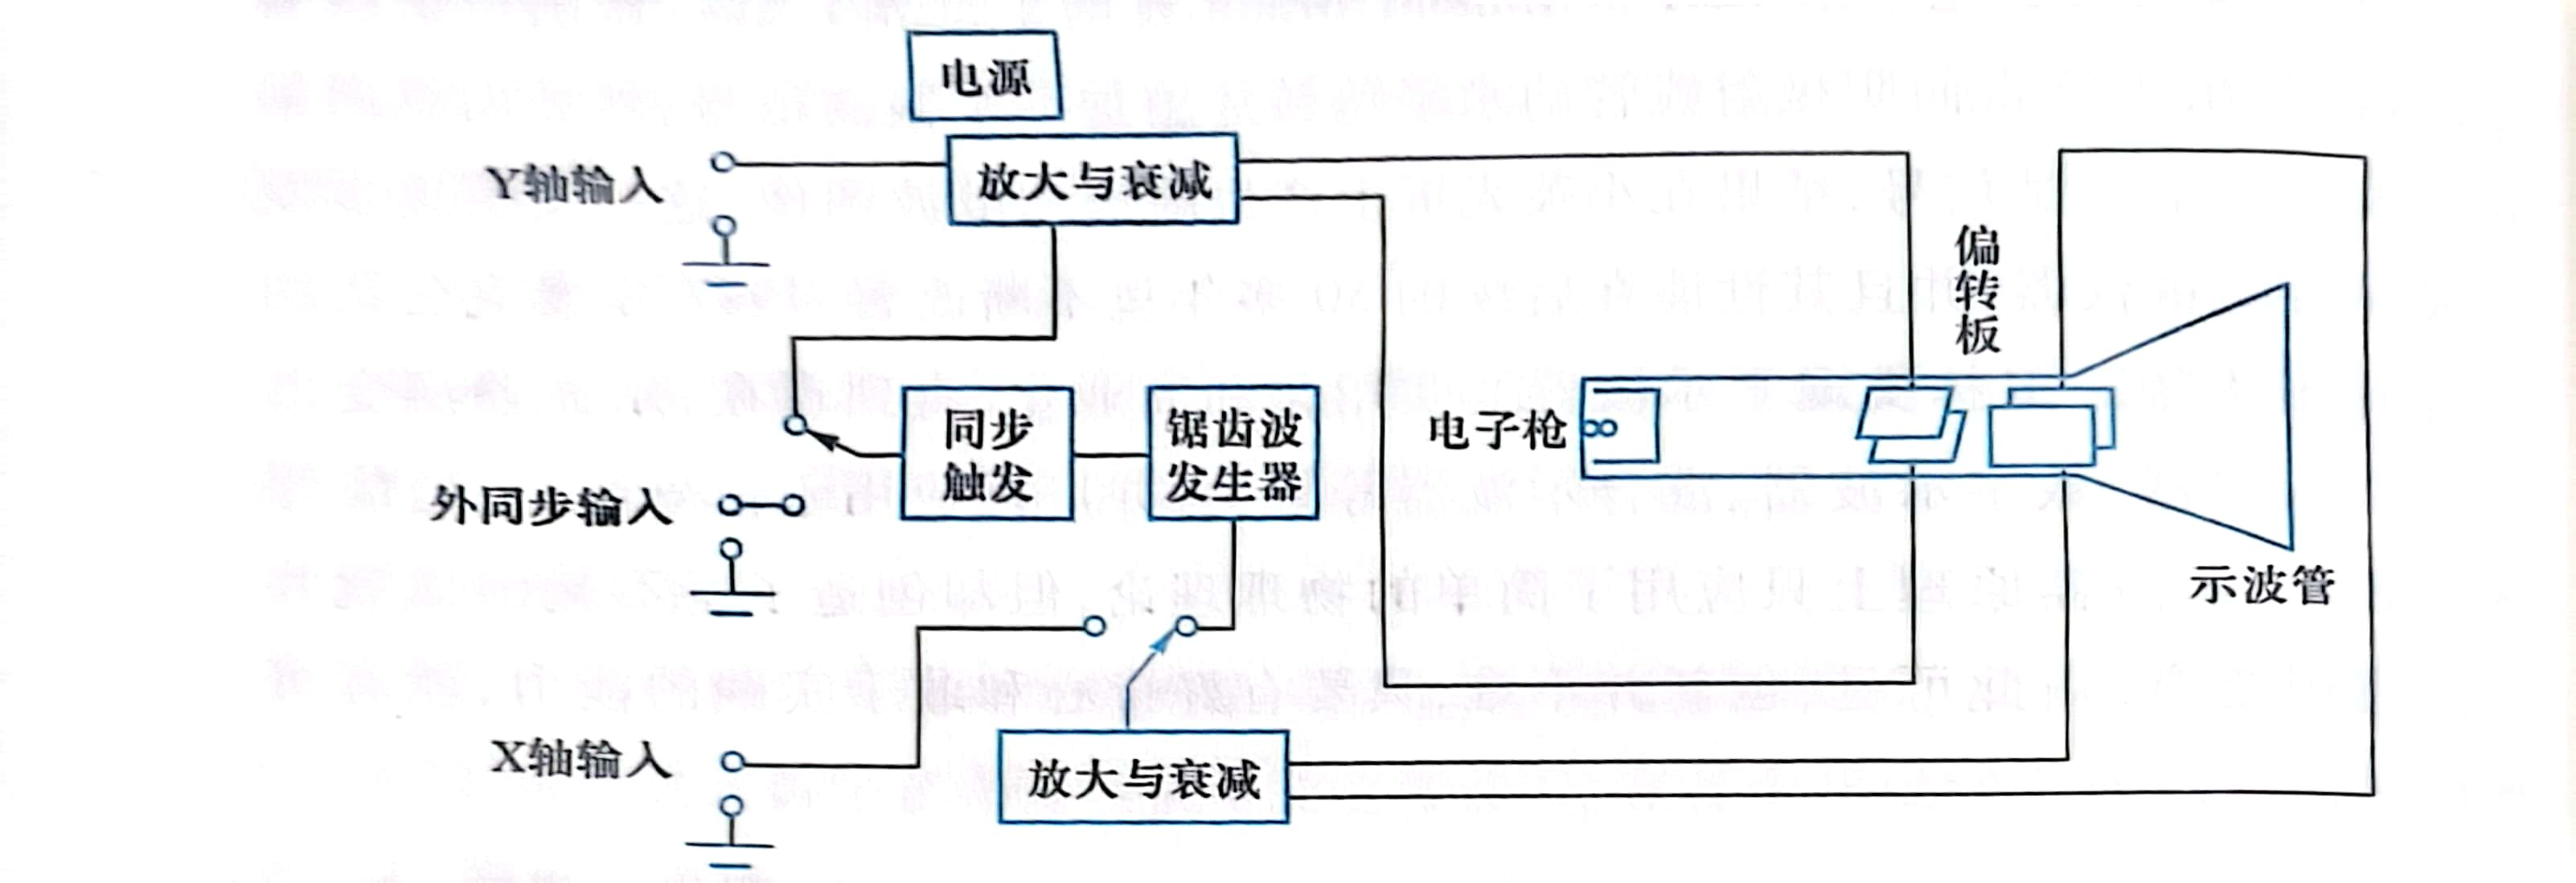
\includegraphics[width=0.9\textwidth,height=0.3\textheight]{monijiegou.jpg}
    \caption{模拟示波器基本结构示意图}
  \end{figure}

  示波管的主要作用是将输入的电信号以二维图形的形式展示出来。示波管主要由电子枪、偏
  转板、显示屏等部分组成,电子枪的作用是向显示屏方向发射大量的电子,这些电子在经过聚焦、
  加速后,再经过水平偏转板和竖直偏转板,轰击到涂有一层荧光物质的显示屏上激发荧光物质发光。竖直
  偏转板通过放大与衰减电路与Y轴输入相连.水平偏转板在示波器的Y-T模式时通过放大与衰减电路与内置的锯齿波
  发生器相连,在示波器的X-Y模式时则与轴输入相连.偏转板在外加电压的作用下可以改变电子束的运动方向,从而在示波
  器上显示输入的信号波形。

  在示波器的控制面板上,“聚焦”旋钮可以调节电子束在显示器上光点的大小;“辉度旋钮”可以调节光点
  的亮度;“Time/DIV”旋钮可以实现信号在X轴上的放大或缩小;“V/DIV”旋钮可以实现信号在Y轴上的放大或缩小。
  示波器工作的Y-T模式与X-Y模式的切换,需要在示波器面板上寻找相应的操作键或旋钮,不同型号的示波器采用不同的方
  法,在使用的时候,可以通过查阅说明书或在示波器面板上寻找“Y一T"符号,再进一步进行模式切换的操作。

  \subsection{示波器的示波原理}
  示波器能使一个随时间变化的电压波形显示在荧光屏上,是靠两对偏转板对电子束的控制来实现的,图\ref{shiboyuanli}显示了
  Y-T模式下波形的显示方式,在图\ref{shiboyuanli}中,左上为输入的Y轴正弦电压信号$u_{y}$。
  它施加在竖直偏转板上;右下为内置的锯齿波电压信号“,它施加在水平偏转板上,
  正弦波电压信号和锯齿波电压信号满足$f_{x}=f_{y}$。在“0”时刻,$u_{x}=u_{y}=0$,
  电子在两极板间电场的作用下偏至左侧,即图\ref{shiboyuanli}中右上方的“0"点位置,随着$u_{x}$,线性增大,电子束
  随时间线性向右偏转,同时在$u_{y}$,作用下向上运动,在“1”时刻,波形运动到右上方“1”的位置,
  进而随时间又运动到“2”、“3”和“4”的位置,从
  而显示出完整的$u_{y}$波形。在这里,电子束从左至右的过程称之为“扫描”。
  \begin{figure}[bt]\label{shiboyuanli}
    \centering
    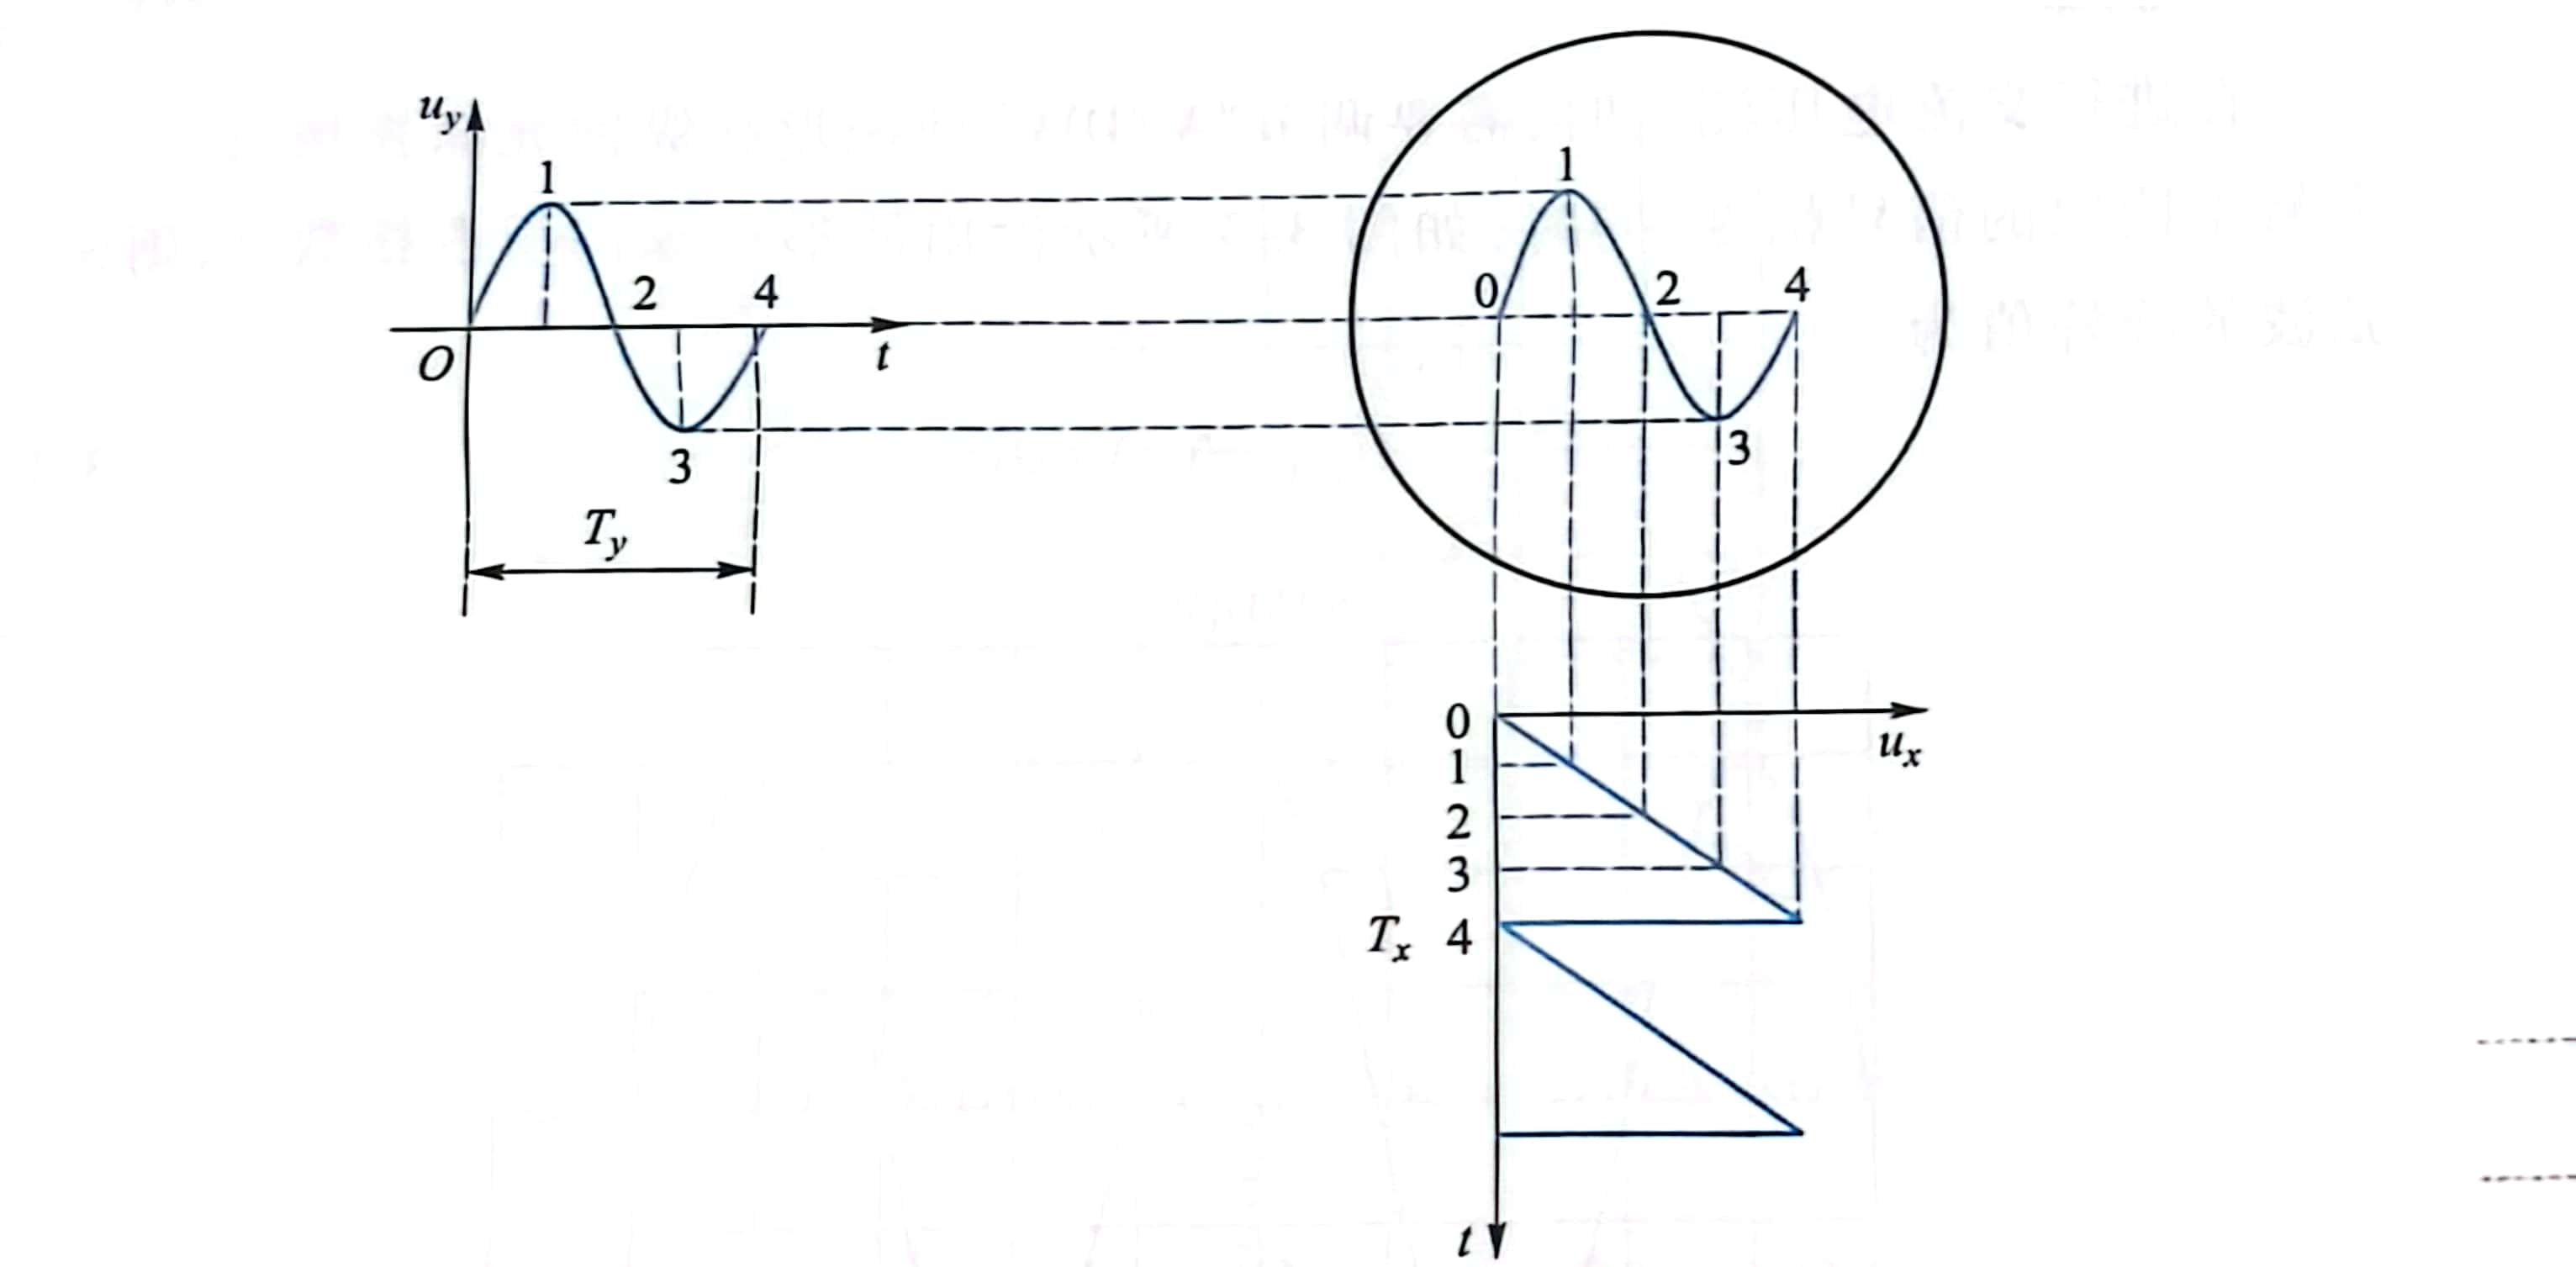
\includegraphics[width=0.9\textwidth,height=0.3\textheight]{shiboyuanli.jpg}
    \caption{示波器的示波原理图解}
  \end{figure}

  \subsection{同步}
  在使用示波器观察和测量信号的时候,一般有“同步”和“触发”两种方式可以使信号在示波器的显示器上稳定显示。

  “同步”指的是被测信号与锯齿波信号同步,此时被测信号的频率$f_{y}$,与锯齿波信号频率$f_{x}$相等或是其
  整数倍,即$f_{y}=nf_{x}$。当满足“同步”条件时,每次锯齿波的扫描起点都能准确地落在被测信号的同一相位点,
  从而使每一次扫描的电子
  束在显示器上形成的轨迹是重合的,显示器能够显示稳定的波形,通过改变示波器上的扫描频率旋钮。
  可以改变扫描频率$f_{x}$,使条件$f_{y}=nf_{x}$满足,如果“同步”条件不能得到满足。
  每一次的扫描起点则会是不同的相位点,于是每次扫出的波形不重复,在这种情况下显示器显示的波形会
  不断地移动.

  “触发”指的是在示波器上设定条件,将被测信号与这些条件对比,当满足条件时,被测信号则开始在显示器上被扫描显示,
  当扫描结束后电路会处于等待状态,直至下一次设定条件满足时开始下一遍的扫描,具体为:使用“触发”功能时,Y轴输入的
  被测信号(内触发)被送至触发电路,当被测信号达到某一选定的触发电平时,触发电路输出触发脉冲启动锯齿波发生器,
  使被测信号从触发电平开始在显示器上被扫描显示,直至一个锯齿波周期结束,
  “触发”保证了每次扫描都会使波形从同一相位点开始显示,因而每次扫描的波形都完全重合。
  在大学物理实验中,一般使用内触发功能,即在实验的时候将“他发源”设定为输人的待测信号。
  之后调整“触发电平”,选择好“上升沿触发”或“下降沿触发”,让触发电平的绝对值不高于待测信号的峰值。

  \subsection{测量}
  在进行交流电压测量时,需要调节“V/DIV”使波形在纵向充满视场,以获得一个易于读取的信号幅度。
  同时,如图\ref{jiaoliuceliang}所示读出波形在纵向所占格数N,则该示弦波的峰峰值为
  \begin{equation}
    U_{P-P}=N \times V/DIV
  \end{equation}

  \begin{figure}[bt]\label{jiaoliuceliang}
    \centering
    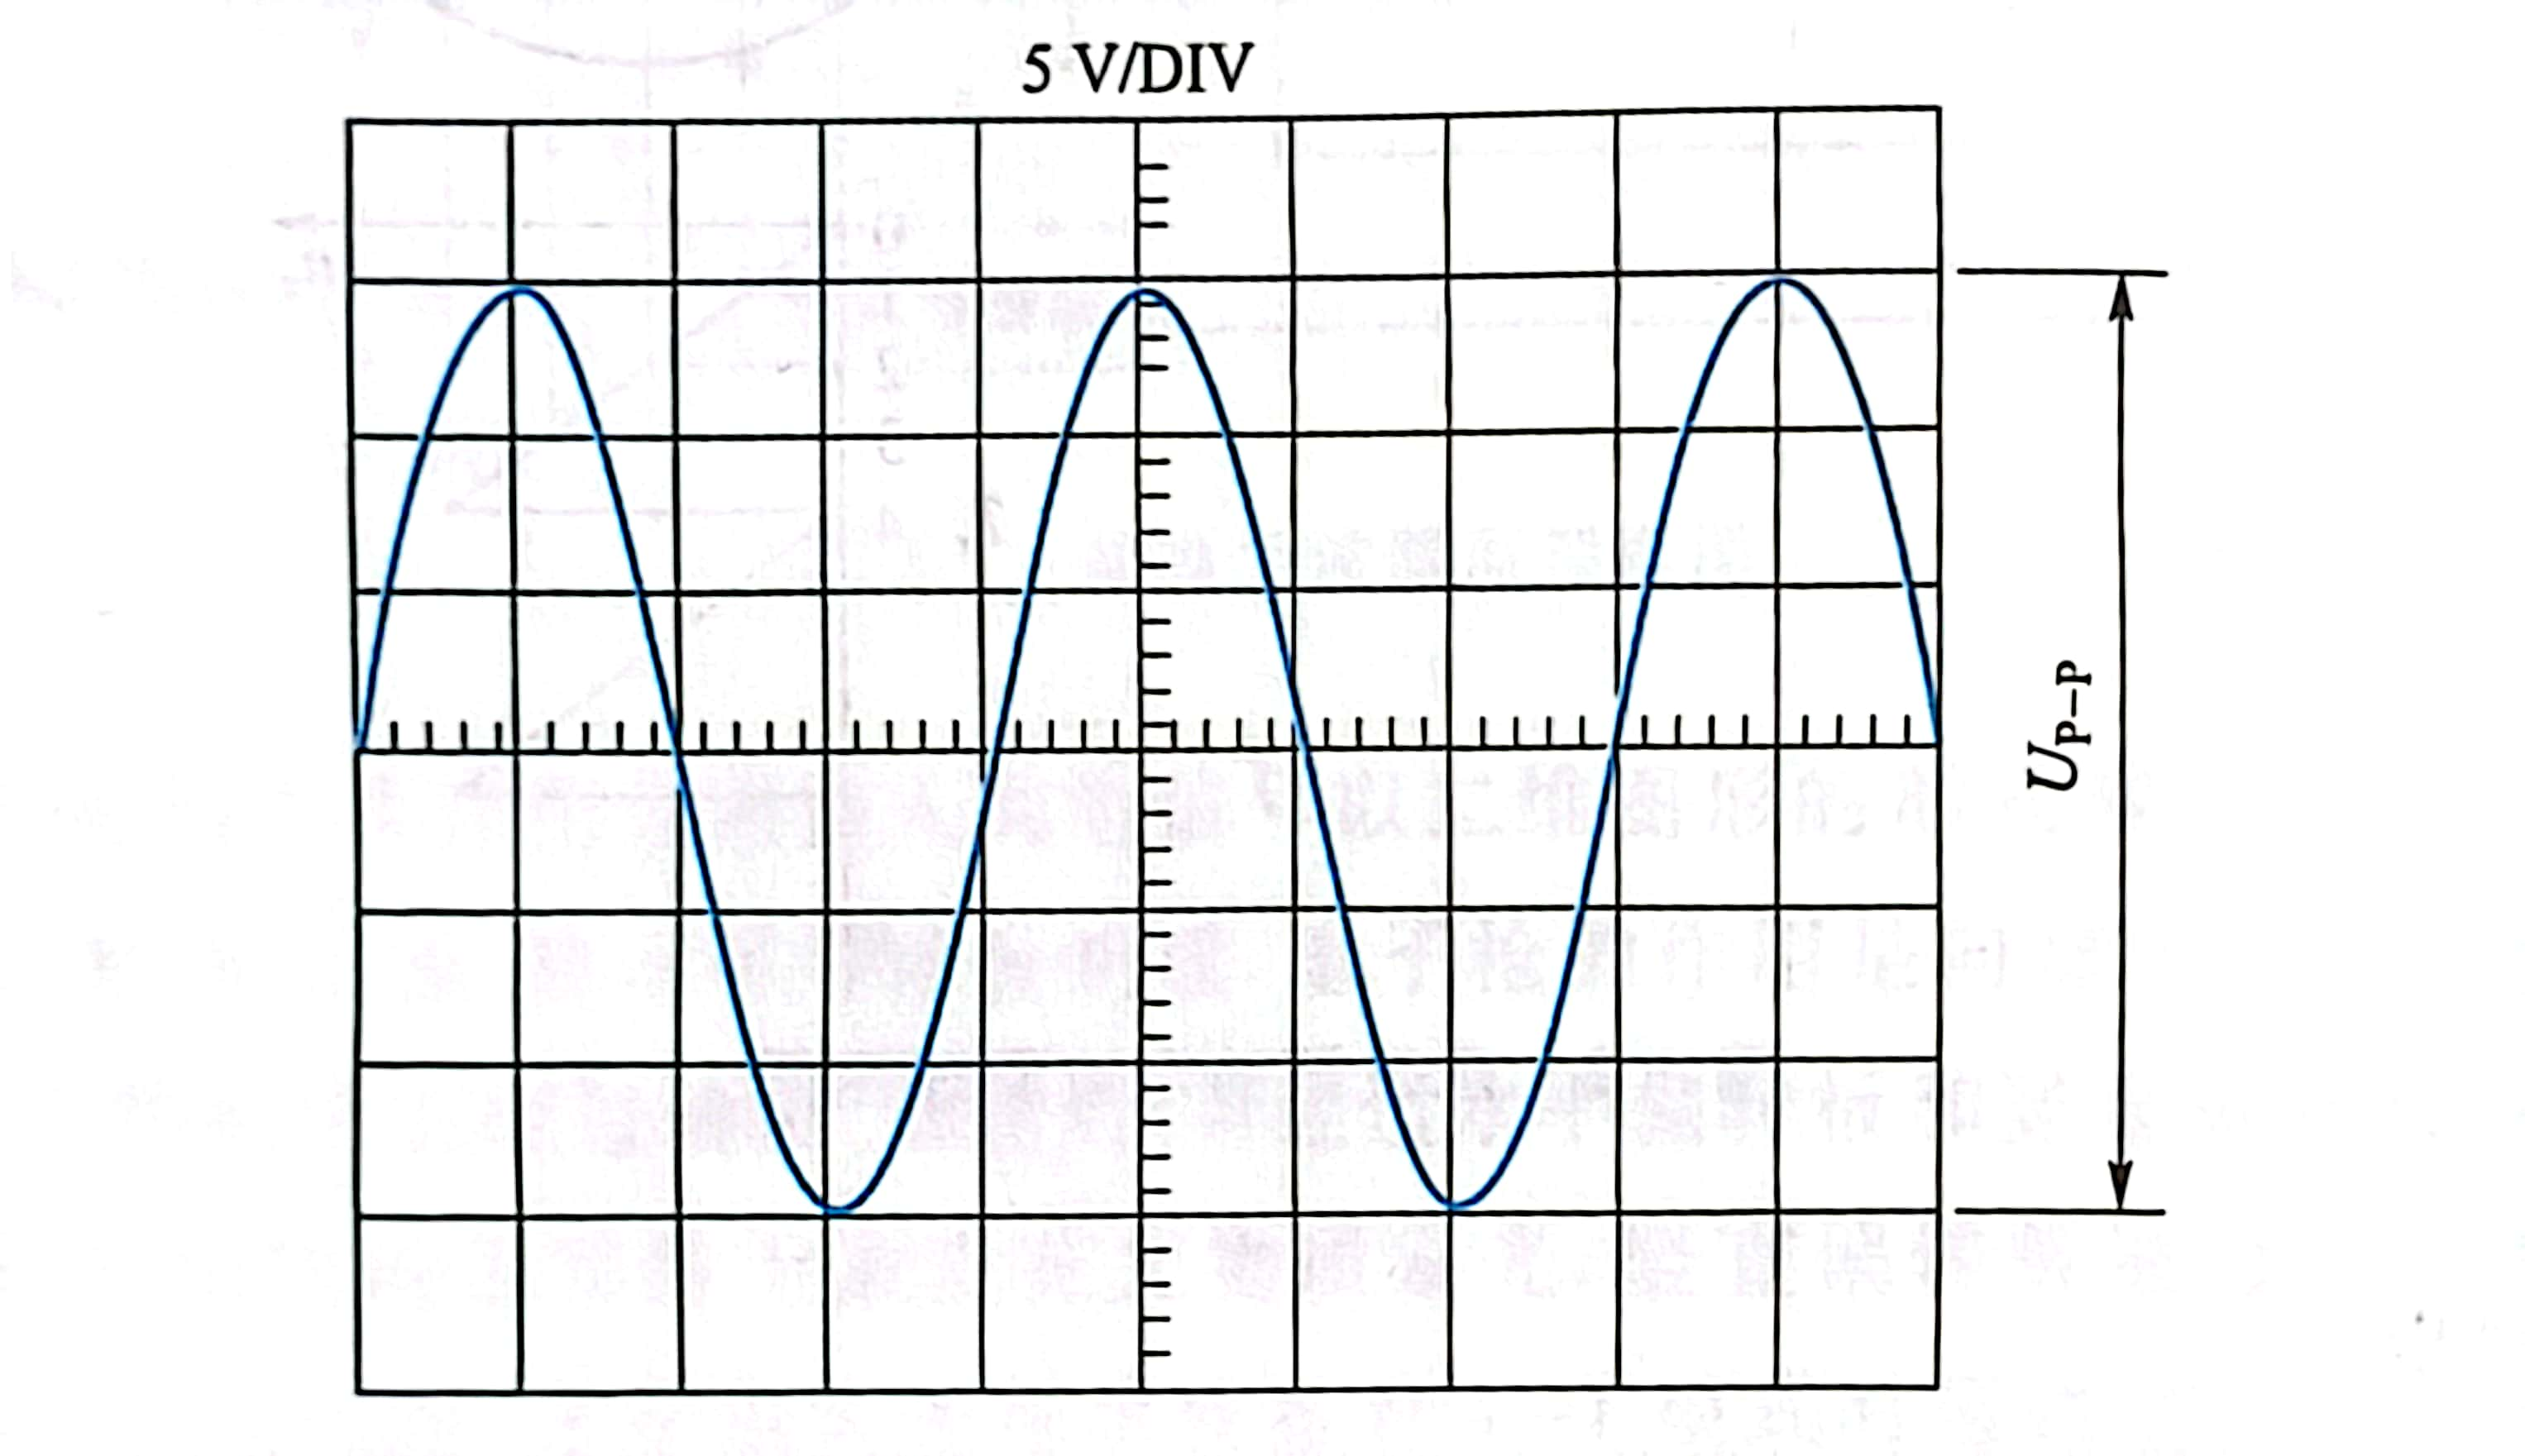
\includegraphics[width=0.9\textwidth,height=0.3\textheight]{jiaoliuceliang.jpg}
    \caption{交流电压测量示意图}
  \end{figure}

  在测量信号频率时,调节Time/DIV,使波形的n个周期充满视场,获得n个周期在X轴方向所占的格数M,则可以得到的信号频率为
  \begin{equation}
    f=\frac{1}{T}=\frac{n}{M\times Time/DIV}
  \end{equation}

  在测量两个信号之间的相位差时,首先需要在示波器的显示屏上稳定显示两个输人信号,
  如图\ref{xiangweichaceliang}所示.读出一个周期所占格数M,再读出两列波相近峰值所跨的格数L,则相位差为
  \begin{equation}
    \Delta \phi =(L/M)\times 360^{\circ} 
  \end{equation}

  \begin{figure}[bt]\label{xiangweichaceliang}
    \centering
    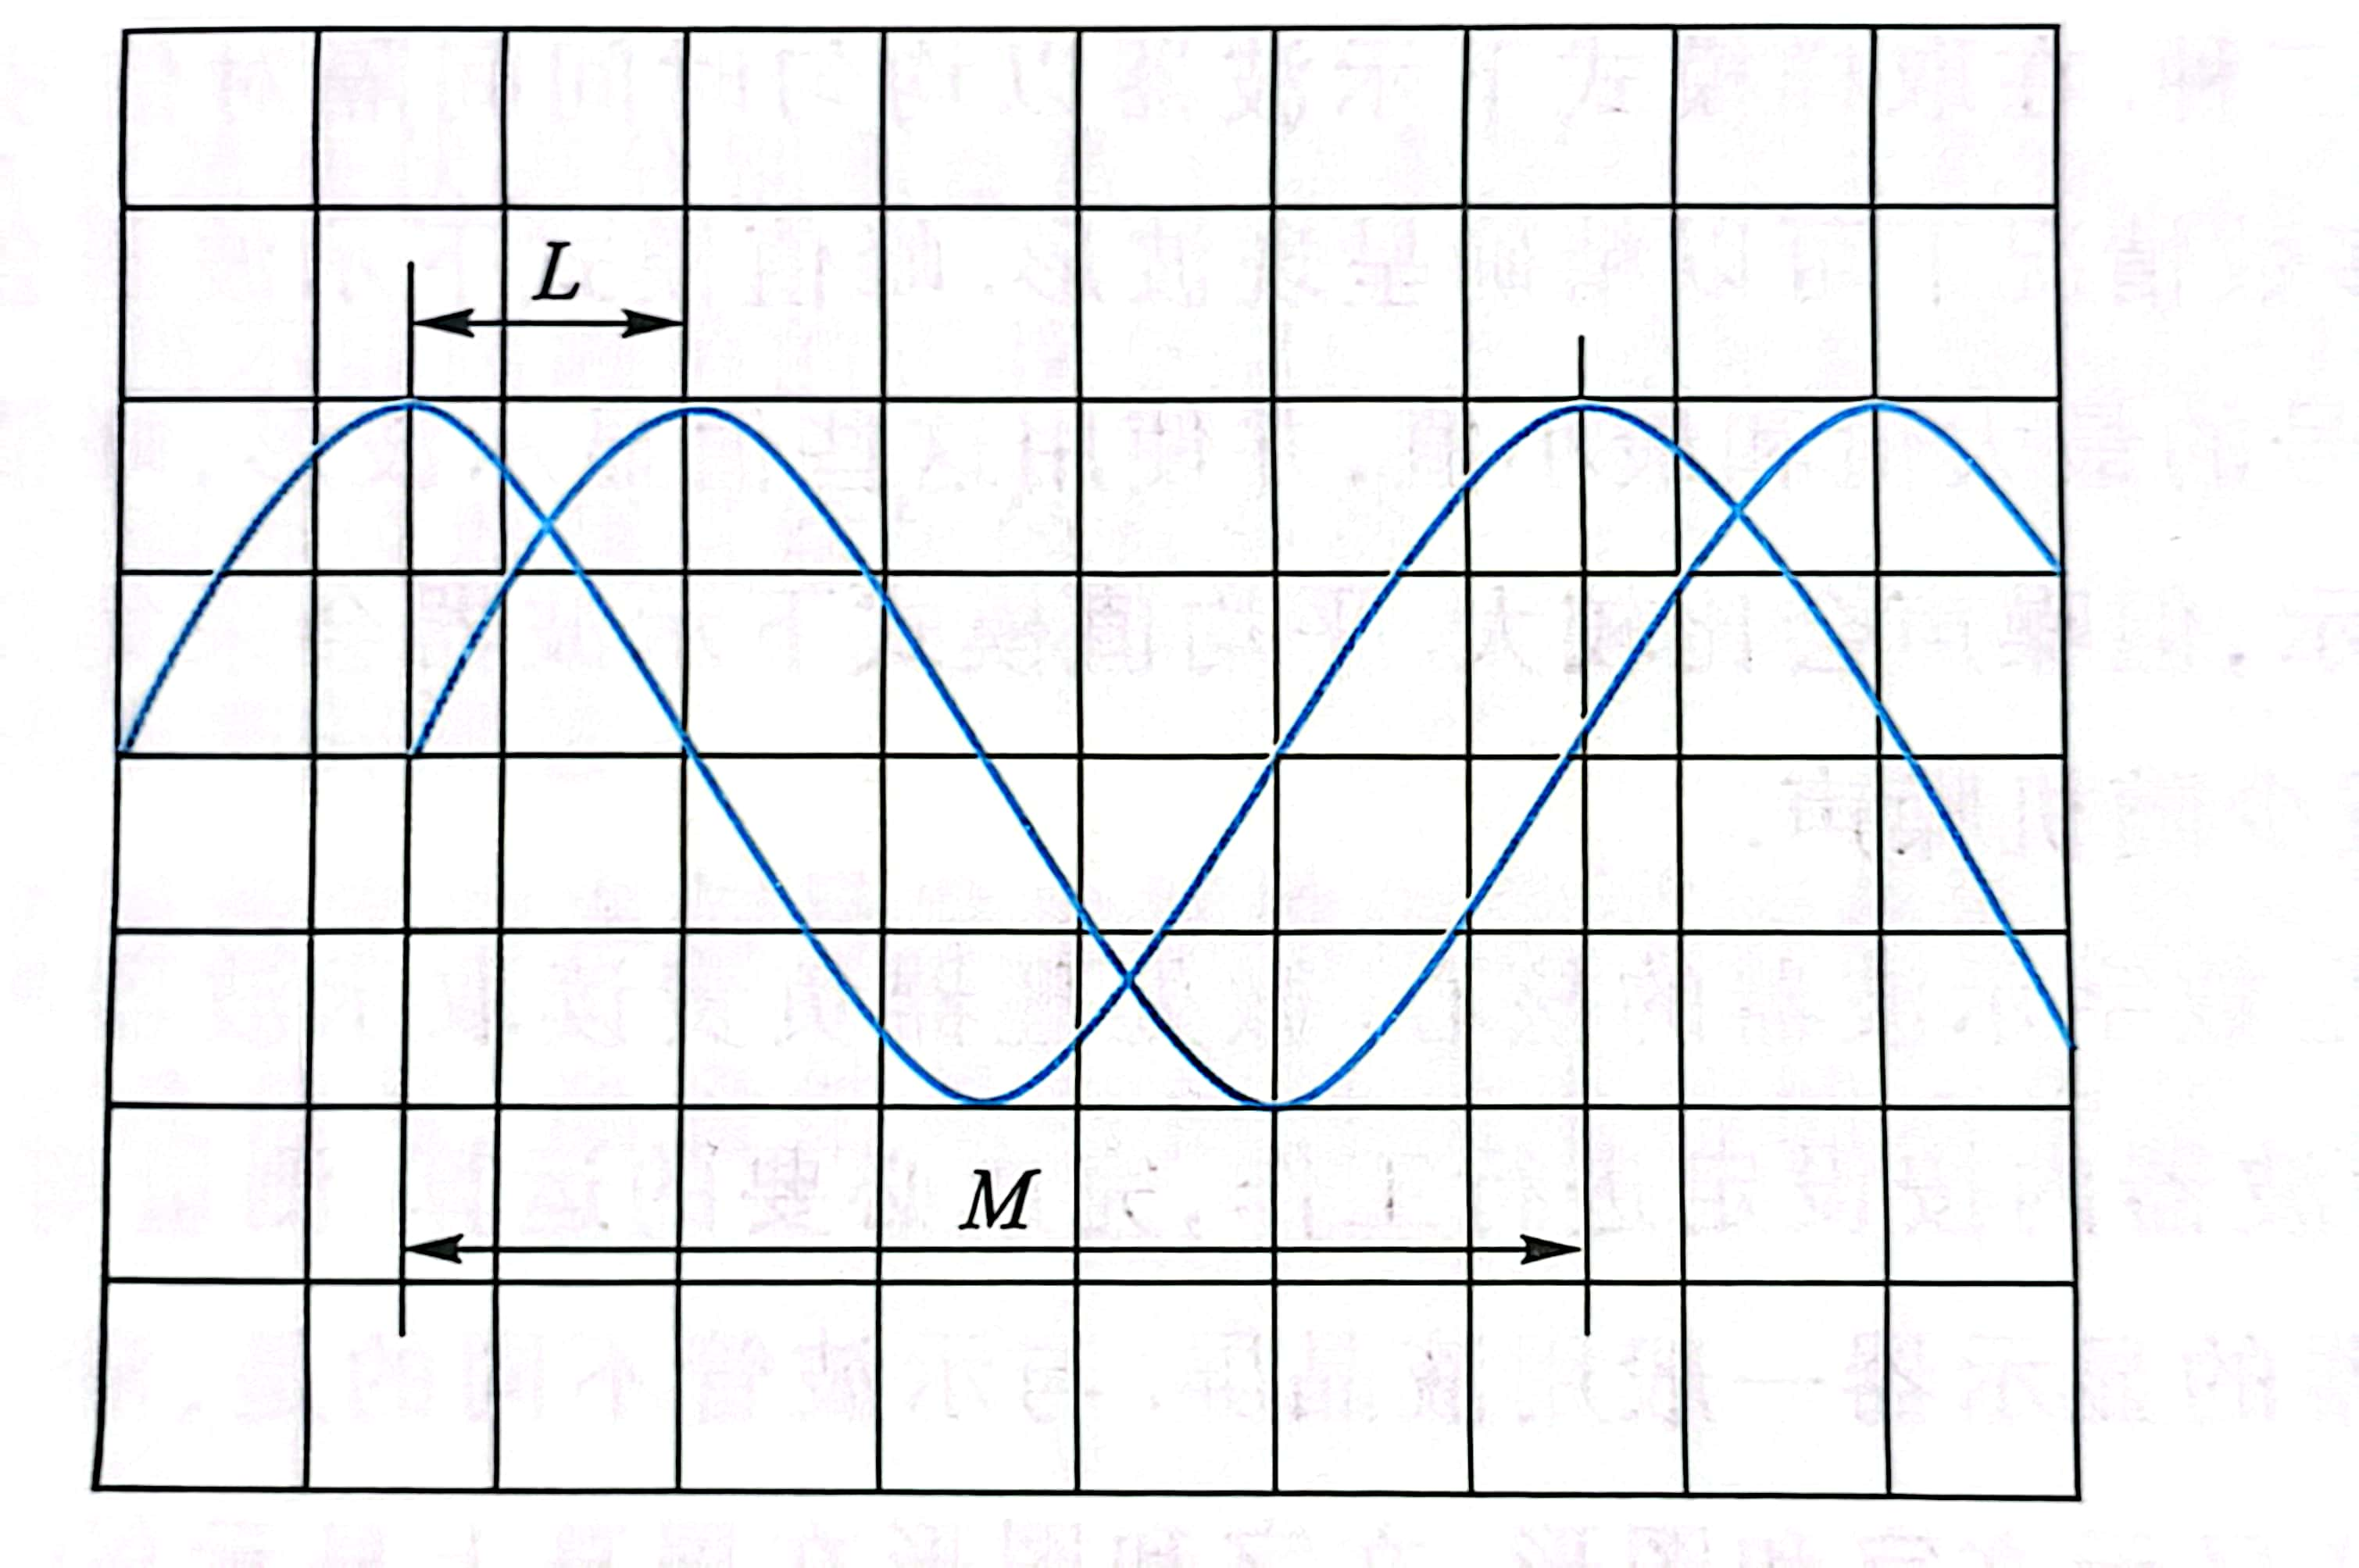
\includegraphics[width=0.9\textwidth,height=0.3\textheight]{xiangweichaceliang.jpg}
    \caption{相位差的测量示意图}
  \end{figure}

  \subsection{观察李萨如图形}
  启动示波器的X-Y开关,此时示波器工作在X-Y方式.X轴信号由CH1输入,Y轴信号由CH2输入.
  在示波器轴和Y轴同时输入不同的正弦信号时,光点的运动是两个相互垂直的简谐振动的合成,
  若它们的频率的比值$f_{x}\mbox{:}f_{y}=\mbox{整数}$时,合成的轨迹是一个封闭的图形,称为李萨如图。
  李萨如图的图形与两信号的频率比和相位差都有关系,李萨如图与两信号的频率比有如下简单的关系:
  \begin{equation}\label{guanxi1}
    \frac{f_{x}}{f_{y}}=\frac{n_{x}}{n_{y}}
  \end{equation}

  式子中的$n_{x}\mbox{和}n_{y}$,分别为李萨如图的外切水平线的切点数和外切垂直线的切点数,如图\ref{lisaru}所示.
  \begin{figure}[H]\label{lisaru}
    \centering
    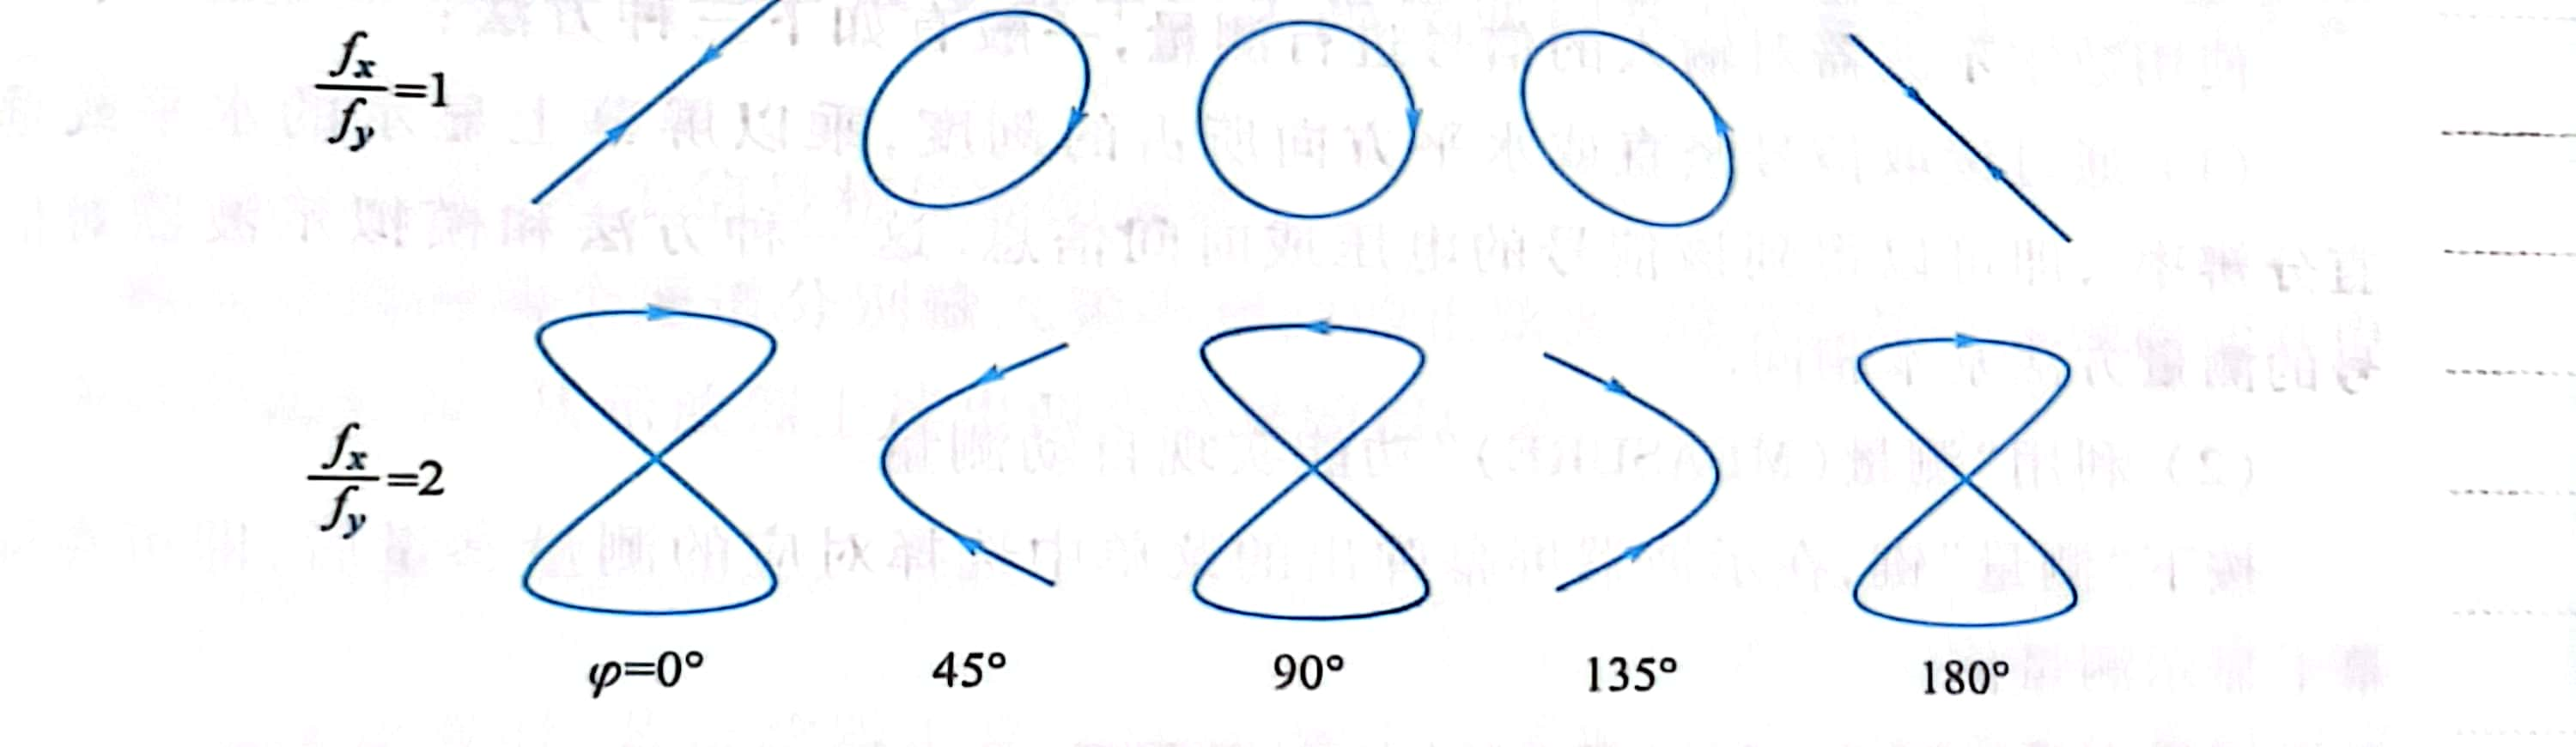
\includegraphics[width=0.9\textwidth,height=0.4\textheight]{lisaru.jpg}
    \caption{李萨如图形}
  \end{figure}
  
  \subsection{数字示波器}
  图\ref{shuzishiboqi}是数字示波器的结构示意图.数字示波器由Y轴的衰减与放大、
  采样与A/D转换、触发电路、输出等几部分组成。数字示波器工作时,待测信号先经过一个电压放大与衰减电路,
  将待测信号放大(或衰减)到后续电路可以处理的范围内,
  接着由采样电路按一定的采样频率对连续变化的模拟波形进行采样,然后由模数转换器A/D将采样得到的模拟量转换成数字量,
  并将这些数字量存放在存储器中。
  这样,可以随时通过CPU 和逻辑控制电路把存放在存储器中的数字波形显示在显示屏上供使用者观察和测量.
  \begin{figure}[H]\label{shuzishiboqi}
    \centering
    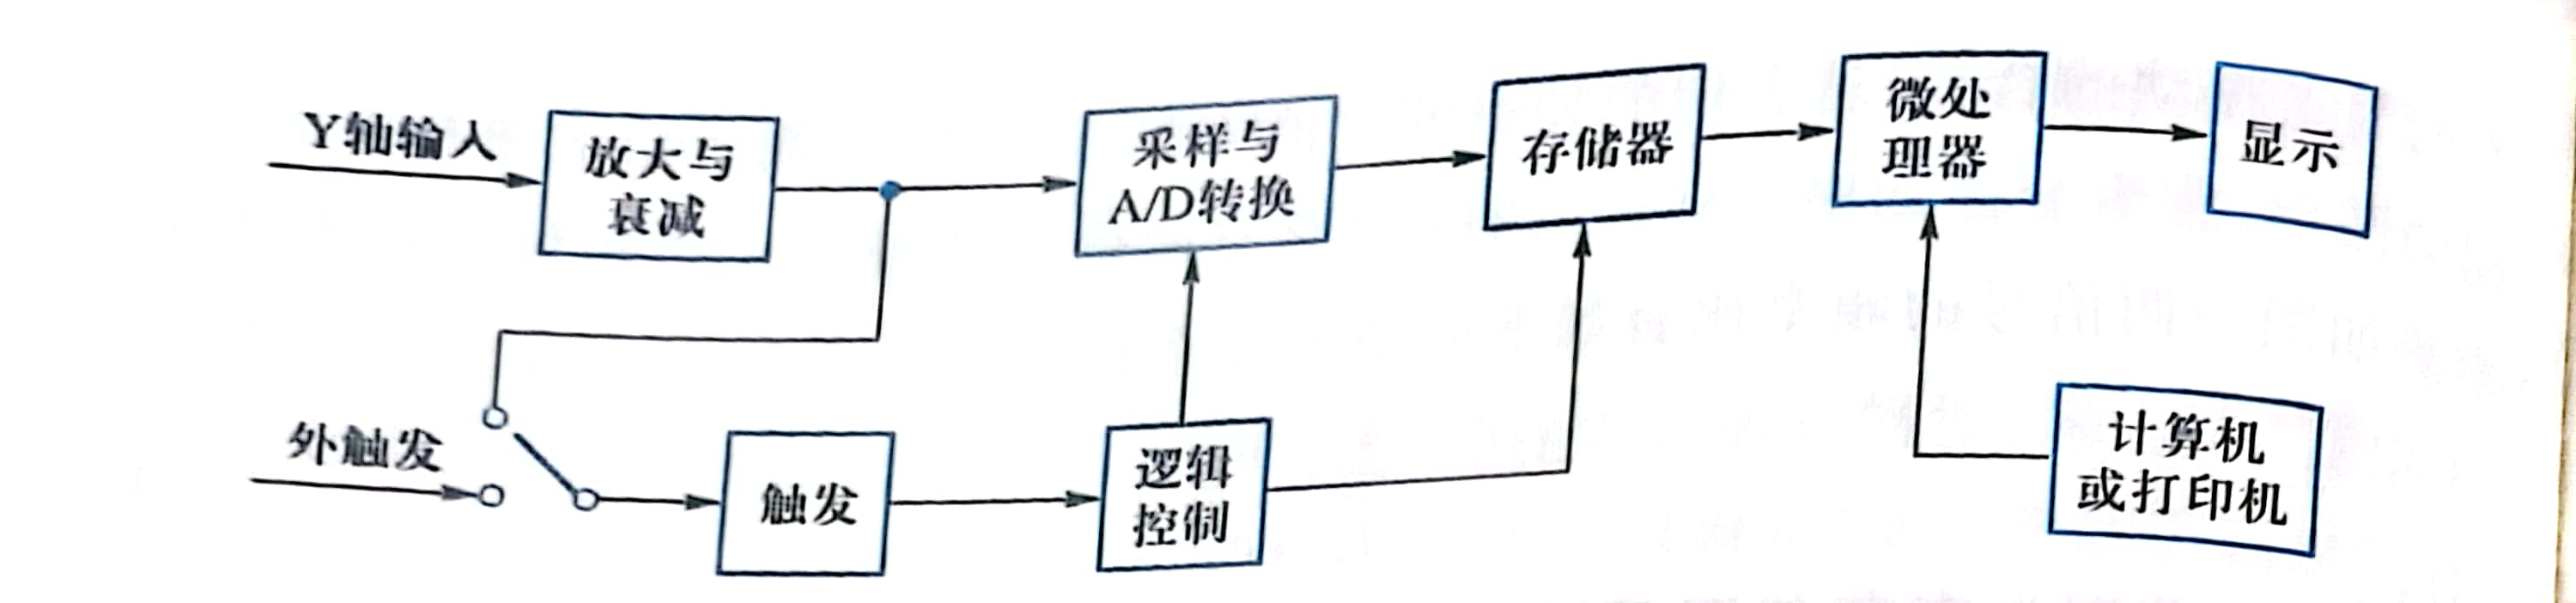
\includegraphics[width=0.9\textwidth,height=0.4\textheight]{shuzishiboqi.jpg}
    \caption{数字示波器结构示意图}
  \end{figure}

  采集信号时,示波器将其转换为数字形式并显示波形,采集模式有取样、峰值检测和平均值三种。
  在取样模式下示波器以均匀时间间隔对信号进行取样以构建波形.此模式多数情况下可以精确呈现波形。
  峰值模式下示波器会在每个取样间隔中找到输入信号的最大值和最小值,并使用这些值显示波形,
  峰值模式有利于窄脉冲的采集和显示,但噪声会比较大.平均值模式下示波器会采集几个波形求平均值再显示,可以减少随机噪声。

  微处理器是数字示波器的核心,微处理器负责读取示波器控制面板上的参数设定,并控制示波器内按设定进行工作,
  完成必要的运算、测量等任务。数字示波器的显示器一般用液晶屏。
  与示波管不同的是:液晶屏是利用单个像素的亮暗状态来显示文字和图形,文字和图形在屏幕上显示的时间可以根据需要进行设定。
  
  使用数字示波器对输入的信号进行测量,一般有如下三种方法:
  (1)通过读取信号竖直或水平方向所占的刻度,乘以屏幕上显示的水平或垂直分辨率,
  即可以得到该信号的电压或时间信息.这一种方法和模拟示波器对信号的测量方法基本相同。

  (2)利用“测量(MEASURE)”功能实现自动测量。按下“测量”键,在示波器屏幕弹出的菜单中选择对应的测量参量后,
  即可在屏幕上显示测量值。

  (3)利用“光标(CURSOR)”功能实现测量按下“光标”键后,示波器的屏幕上出现X轴或Y轴方向的光标线,
  并在显示器上显示两根光标线之间的电压或时间信息.移动光标线至测量点即可获得测量值。

\section{实验装置器材介绍}
双踪示波器、数字功率信号发生器、交流毫伏表、导线等

\section{实验内容及实验步骤}
  \subsection{示波器的初调}
  将示波器自带的校正信号输入到示波器的“Y轴输入”端,调节示波器的触发功能。
  使荧光屏上出现稳定的波形,体会“他发源”、“触发电平”和“上升(下降)沿触发”等功能的意义,
  测量校正信号的频率和幅度,并与校正信号的标准值进行对比。

  调节数字功率信号发生器输出方波和三角波,用示波器观察输出波形。

  \subsection{信号电压有效值的测量}
  调节数字功率信号发生器输出正弦波,并接示波器的“Y轴输入”端,调整触发使波形稳定。

  使用示波器和交流毫伏表分别测量数字功率信号发生器输出信号电压的有效值。
  要求至少测量三组不同峰峰值的正弦交流信号。测量结果与信号发生器的示值进行对比,分别分析两种仪器测量结果的百分差。

  \subsection{信号周期和频率的测量}
  调节数字功率信号发生器输出正弦波,并接示波器的“Y轴输入”端,调整触发使波形稳定。

  使用示波器和交流毫伏表分别测量数字功率信号发生器输出信号电压的有效值,
  要求至少测量三组不同峰峰值的正弦交流信号,测量结果与信号发生器的示值进行对比,
  分别分析两种仪器测量结果的百分差.

  \subsection{观察李萨如图像}
  在示波器的两个通道分别输入频率不同,初相位相同的正弦波,观察李萨如图形,
  验证式\ref{guanxi1},改变其中一个正弦波的相位,观察李萨如图形的变化。
\newpage

\section{实验原始数据}
\begin{figure}[H]
  \centering
  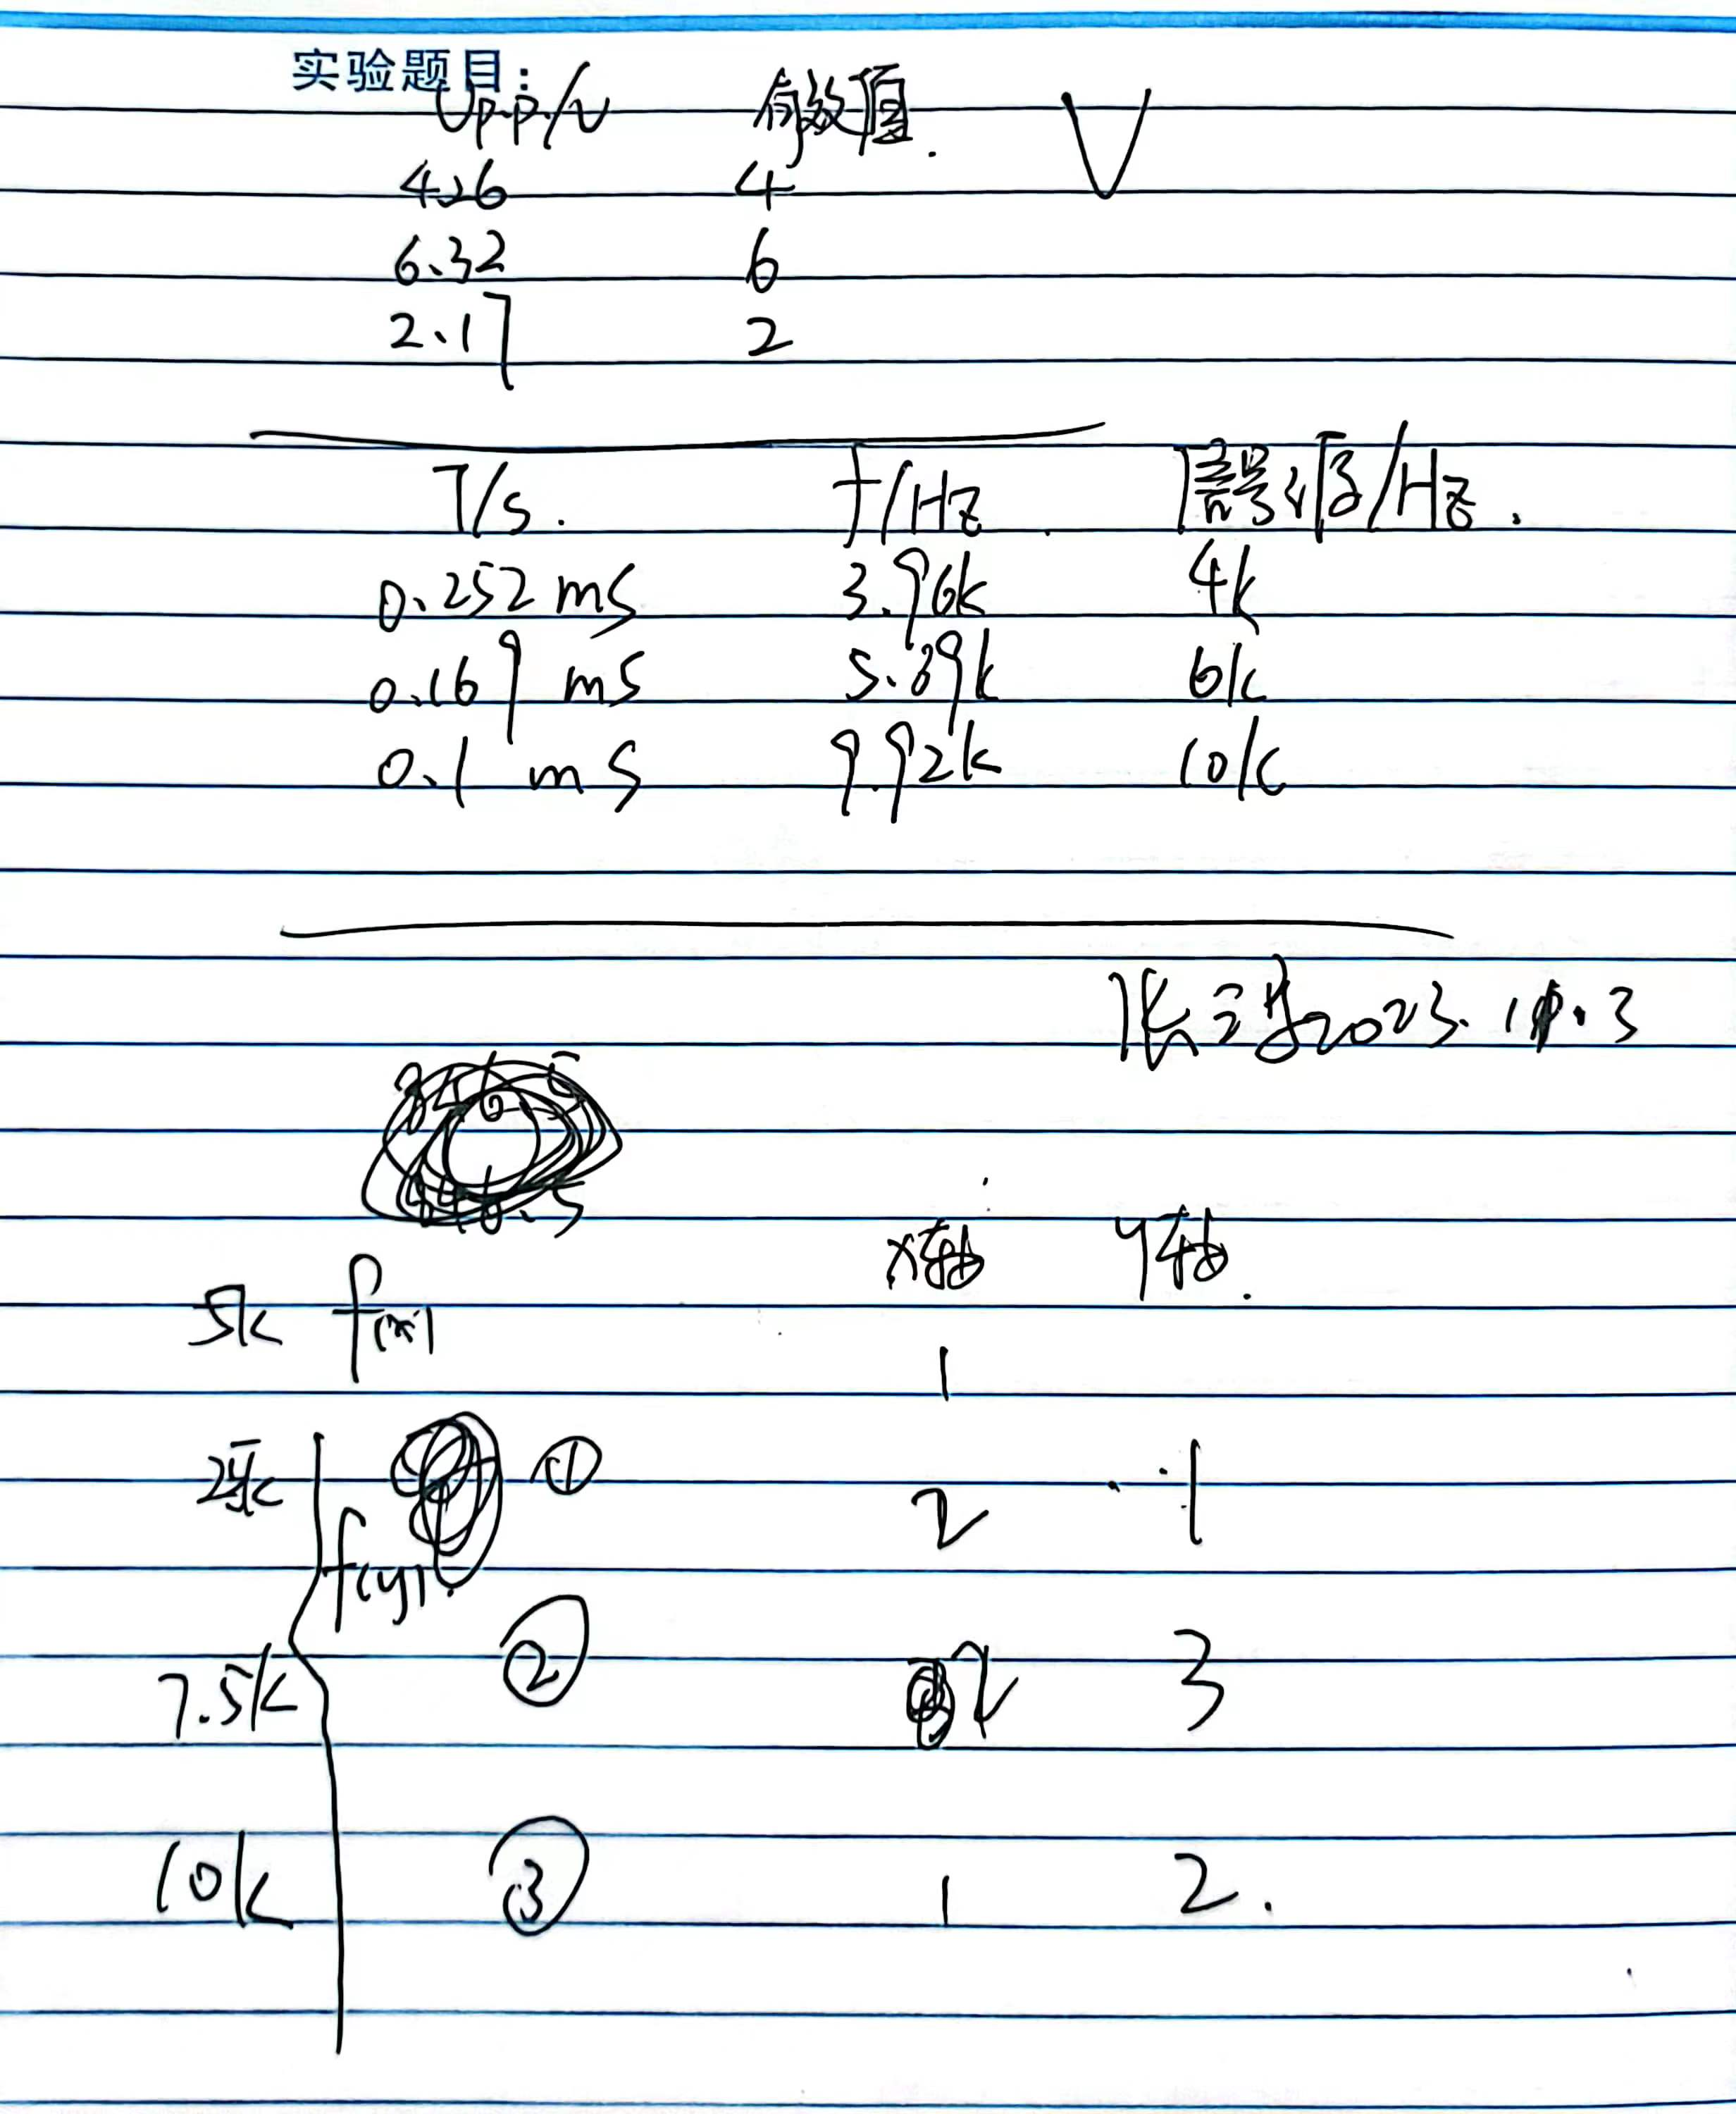
\includegraphics[width=0.9\textwidth,height=0.8\textheight]{shiyanshujv.jpg}
  \caption{实验原始数据}
\end{figure}
\newpage

\begin{figure}[H]
  \centering
  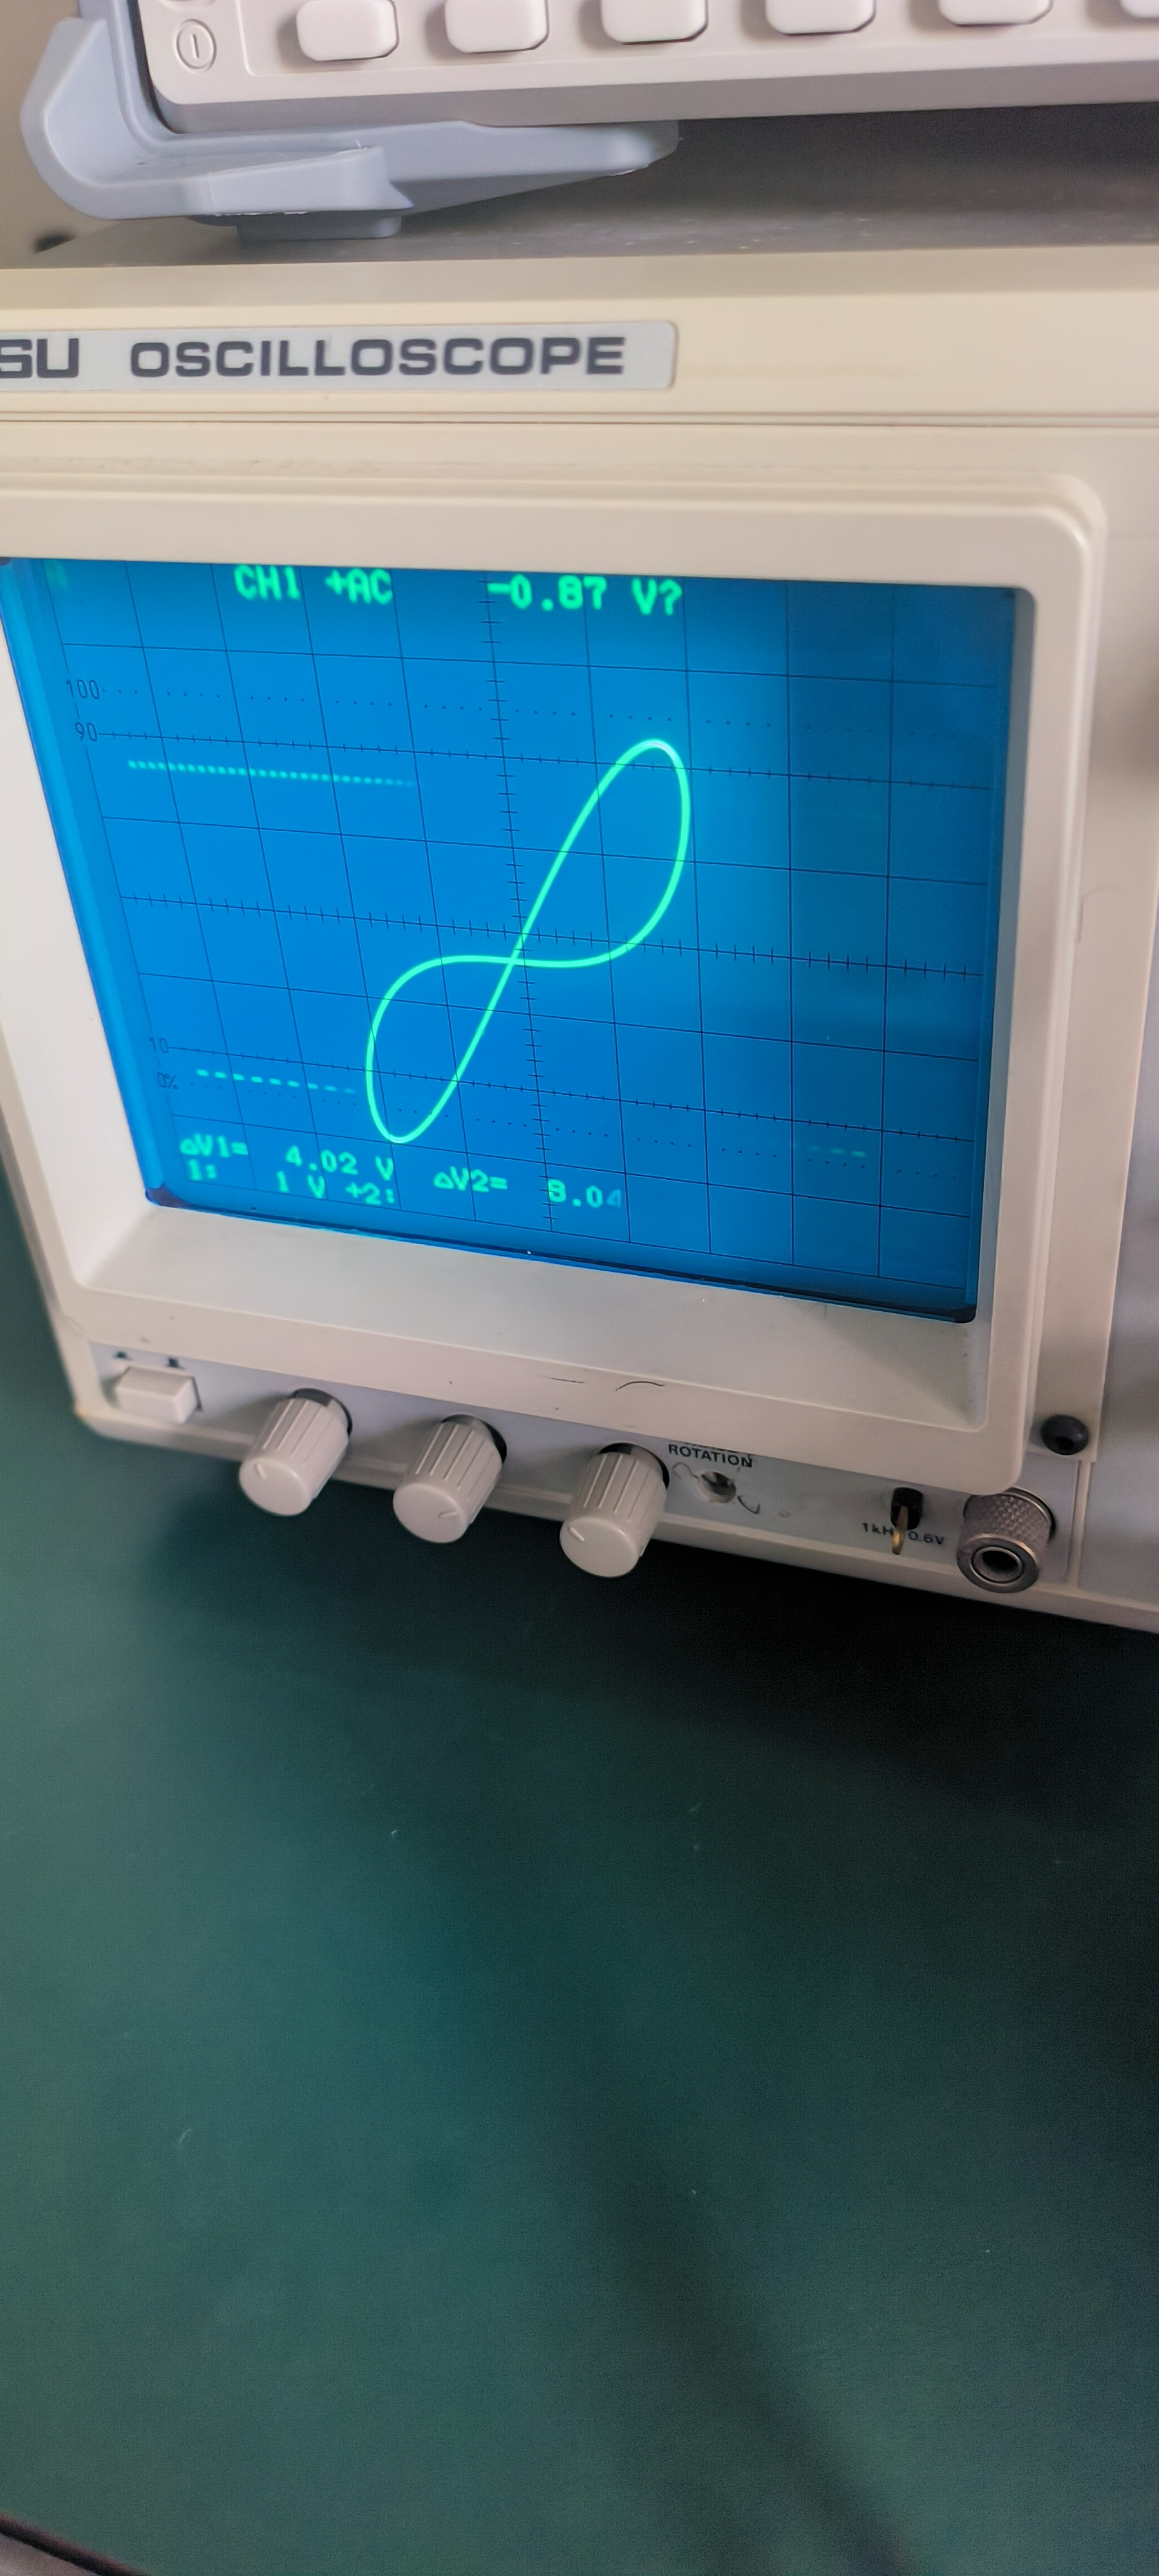
\includegraphics[width=0.6\textwidth,height=0.3\textheight]{shiyanjilu1.jpg}
  \caption{实验记录1}
\end{figure}
\begin{figure}[H]
  \centering
  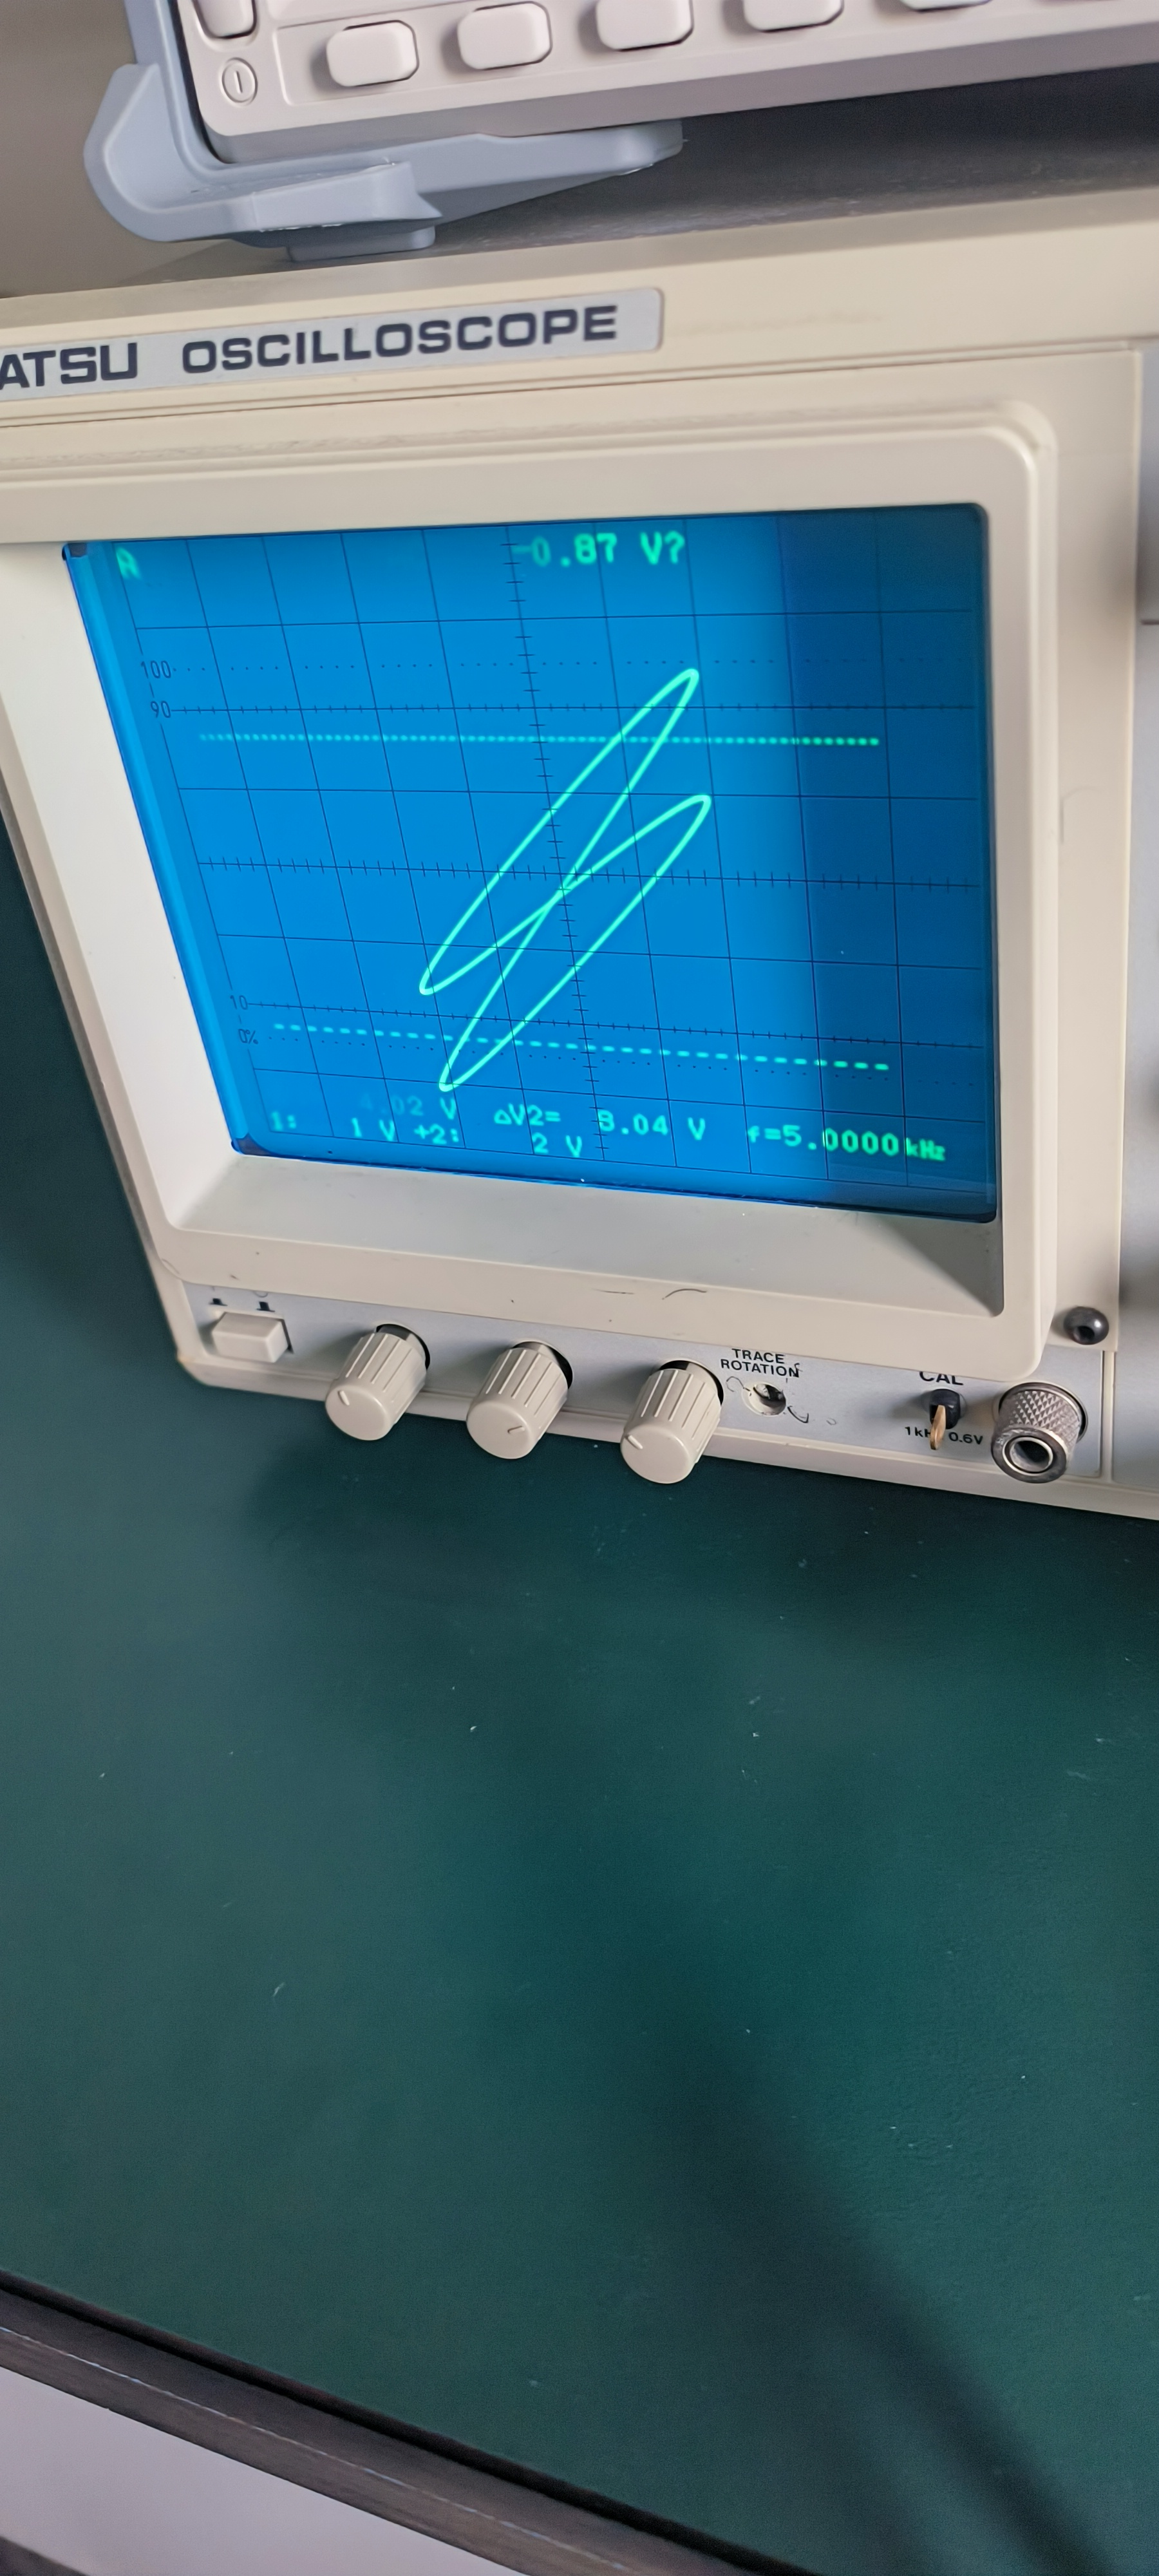
\includegraphics[width=0.6\textwidth,height=0.3\textheight]{shiyanjilu2.jpg}
  \caption{实验记录2}
\end{figure}
\begin{figure}[H]
  \centering
  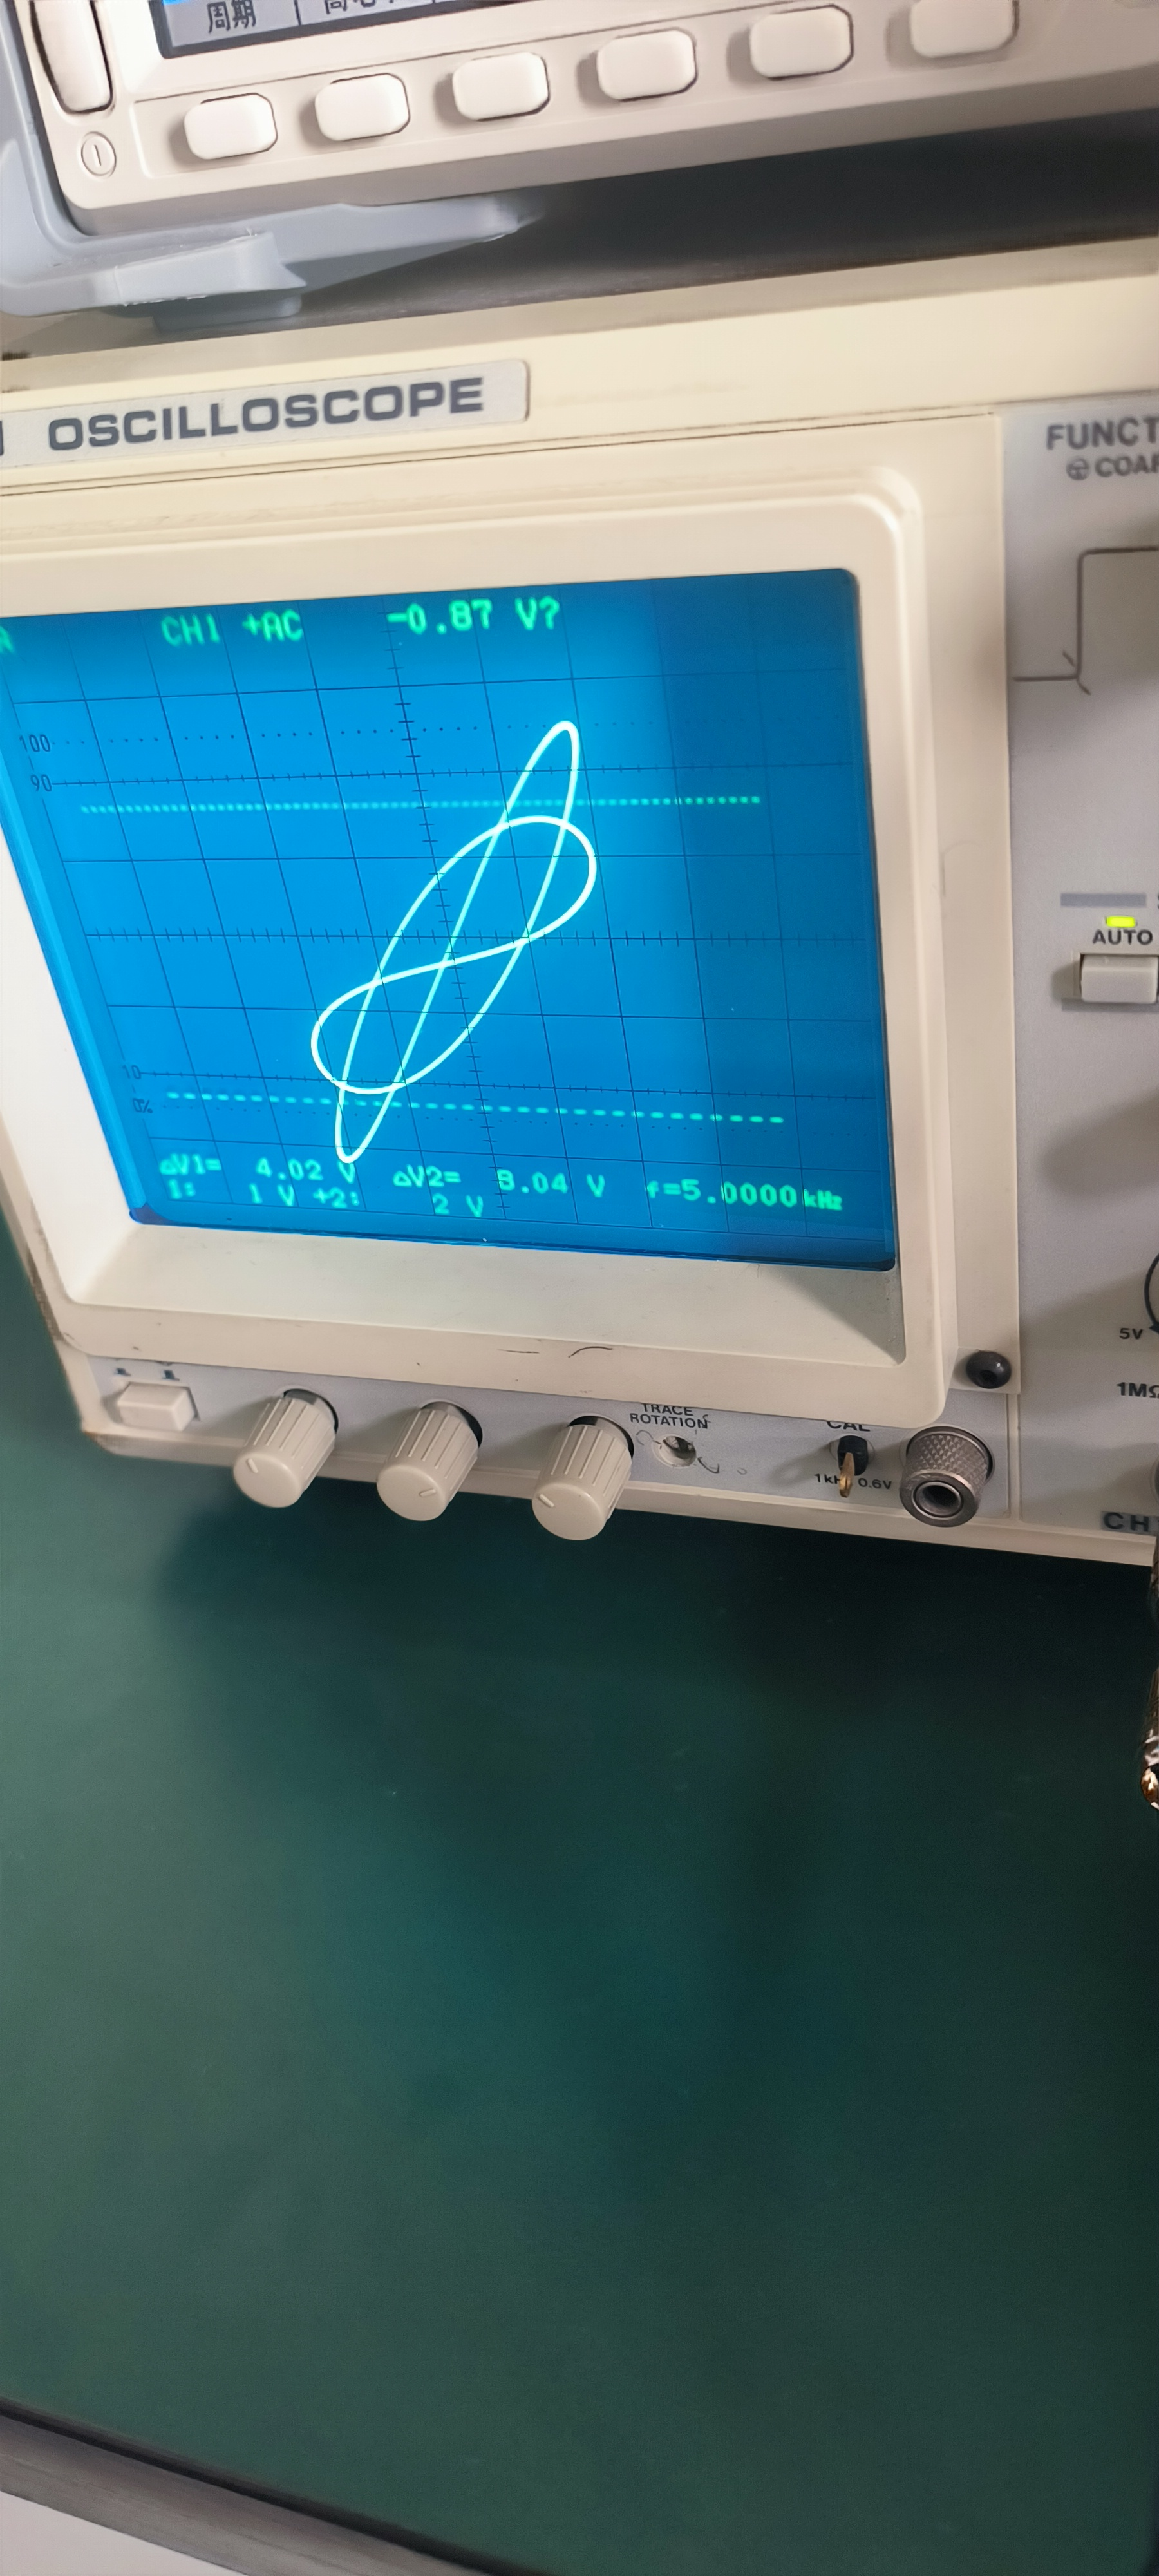
\includegraphics[width=0.6\textwidth,height=0.3\textheight]{shiyanjilu3.jpg}
  \caption{实验记录3}
\end{figure}
\newpage

\section{实验数据处理}
  \subsection{测量RLC串联电路的幅频特性和相频特性}
  \subsection{测量回路的品质因数Q值}

\section{思考题}
  \subsection{思考题一}
  \subsection{思考题二}
  \subsection{思考题三}

\section{实验中个人的思考与感想}
  \subsection{对于实验个人观点}
  \subsection{实验中的总结}

\end{document}
